%-------------------------------------------------------
\begin{frame}{Introduction}{A general view about the Data Mining process}
%-------------------------------------------------------
	\begin{centering}
		\vspace{0.2cm}
		\hspace{-0.2cm}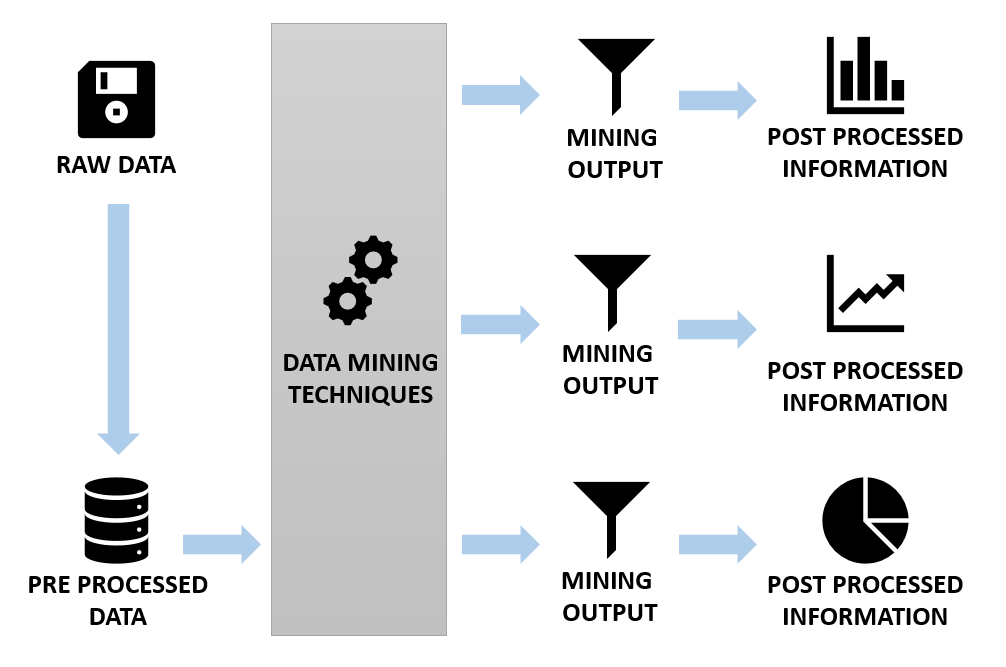
\includegraphics[scale=0.25]{img1_noback.png}
	\end{centering}
\end{frame}

%-------------------------------------------------------
\begin{frame}{Introduction}{The choice of appropriate technologies}
%-------------------------------------------------------

	\centering\textit{Which technology should be employed?} \vspace{0,3cm}

	\begin{block}{}
	    \begin{itemize}
		    \item<1-> \alert{Data Processing}: \hspace{0.2cm} 
\includegraphics[scale=0.18, trim=0 0.8cm 0 0]{../thesis/img/mongodb.png} \\\vspace{0.2cm} \emph{New tech, noSQL paradigm, good skill to learn!} \vspace{0.4cm}
		    \item<2-> \alert{Data Mining}: \hspace{0.2cm} 
\includegraphics[scale=0.18, trim=0 0.8cm 0 0]{../thesis/img/weka_noback.png}
			\item<3-> \alert{Visualization Techniques} \\
			--- \textbf{R language}: programming language with an extensive data visualization library; \\
			--- \textbf{Spreadsheets}: tabular data managing software, like Microsoft Excel and OpenOffice Calc.
	    \end{itemize}
    \end{block}

\end{frame}
